\documentclass[review]{elsarticle}

\usepackage[utf8]{inputenc}
\usepackage[T1]{fontenc}
\usepackage{amsmath,amssymb}
\usepackage{graphicx}
\usepackage{booktabs}
\usepackage{multirow}
\usepackage{hyperref}
\usepackage{xurl}
\usepackage{lineno}
\usepackage{siunitx}

\linenumbers

\journal{Transportation Research Part D}

\begin{document}

\begin{frontmatter}

\title{Precipitation Sensitivity of Road Speeds on the UK Strategic Road Network}

\author[cam]{Yibin Li}
\author[cam]{Li Wan\corref{cor1}}
\cortext[cor1]{Corresponding author}
\ead{lw432@cam.ac.uk}

\affiliation[cam]{organization={Department of Land Economy, University of Cambridge},
            city={Cambridge},
            postcode={CB3 9EP},
            country={United Kingdom}}

\begin{abstract}
Precipitation reduces road traffic speeds, yet link-level evidence on how individual road segments respond to rainfall remains scarce. We develop a three-stage Estimate--Map--Explain framework and apply it to approximately 9~million hourly observations from 460 Strategic Road Network links in Cambridgeshire, UK (2022--2024). A Gamma generalised linear model with link-specific precipitation interactions reveals that sensitivity varies by an order of magnitude across links: motorway segments show near-zero effects while single-carriageway connectors experience speed reductions up to four times the network baseline of 2.1\% per mm\,hr\textsuperscript{$-$1}. A weighted least squares regression identifies lanes, speed limit, daily flow, and rural classification as significant predictors, explaining 34\% of the cross-link variation. Betweenness centrality analysis identifies segments where individual vulnerability and network importance compound. The framework uses only publicly available data, runs on a standard laptop, and is released as an open-source platform.
\end{abstract}

\begin{keyword}
precipitation sensitivity \sep road traffic speed \sep Gamma GLM \sep Strategic Road Network \sep link-level heterogeneity \sep betweenness centrality \sep climate adaptation
\end{keyword}

\end{frontmatter}

%% ---- HIGHLIGHTS (for TRD submission) ----
%% 3--5 bullets, each max 85 characters including spaces
\noindent\textbf{Highlights}
\begin{itemize}
\item Link-level precipitation sensitivity varies tenfold across 460 SRN segments
\item Gamma GLM on 9 million observations yields 460 road-specific coefficients
\item Lanes, speed limit, flow and rural class explain 34\% of the variation
\item Centrality analysis identifies compounding vulnerability on A14 corridor
\item Open-source platform enables replication by any local transport authority
\end{itemize}


%% ============================================================
%% 1. INTRODUCTION
%% ============================================================
\section{Introduction}
\label{sec:intro}

Climate change is intensifying the hydrological cycle across the United Kingdom, with precipitation extremes projected to increase by 10--30\% under high-emission scenarios by 2070 \citep{ukcp18,stern2007contribution,koetse2009impact}. For the Strategic Road Network (SRN)---the motorways and major A-roads managed by National Highways---these trends translate into operational disruptions: reduced vehicle speeds, increased journey-time variability, and elevated accident risk during wet conditions \citep{hranac2006empirical,maze2006weather,elfaouzi2012effects}. A recent audit found that only 7\% of the SRN meets climate adaptation standards established two decades ago \citep{nce2026srn}, while National Highways' own assessments classify 36\% of the network as having significant flood susceptibility \citep{nh2024climate}. The Department for Transport's Rapid Evidence Assessment explicitly notes that empirical tools linking weather to road transport disruption are largely absent for the UK road network, in contrast to rail where such tools exist \citep{dft2024rea}. These figures underscore an urgent need for evidence-based methods that can quantify how individual road segments respond to precipitation and identify which segments are most vulnerable.

Addressing this need is complicated by two features of the current methodological landscape. On the one hand, the dominant simulation-based approaches---agent-based microsimulation models requiring origin--destination matrices and behavioural calibration \citep{huang2022overview,he2026flood}, and coupled flood-traffic models linking flood inundation with traffic assignment \citep{pregnolato2017depth,pregnolato2016impact,farahmand2024integrating}---offer high-fidelity representations of traffic dynamics but demand substantial data, computational resources, and city-specific calibration. These tools remain inaccessible to most local transport authorities \citep{unece2024stress}. On the other hand, the empirical literature on rainfall--speed relationships, though well-developed at aggregate levels \citep{hranac2006empirical,becker2026rainfall,bi2022weather,cai2016rainfall,koetse2009impact}, overwhelmingly reports network-wide or corridor-level average effects. Such averages mask the heterogeneity that exists between individual road segments and cannot support targeted adaptation investment.

A small but growing body of work has begun to explore link-level variation. \citet{gao2024resilience} used hierarchical clustering to group road segments by resilience pattern based on road environment variables, revealing meaningful heterogeneity in rainfall response across a Chinese expressway network. \citet{li2024percolation} applied percolation theory to highway networks under rainfall, demonstrating that network connectivity degrades non-linearly as precipitation intensity increases. \citet{liu2026extreme} integrated multiple impact factors and delay propagation to model road transport resilience under extreme rainfall in Cambridge. However, none of these studies combines link-level empirical estimation of rainfall sensitivity with a regression-based identification of which road characteristics systematically drive the observed variation---the step needed to generate actionable guidance for infrastructure planners.

This paper addresses these gaps through a three-stage analytical framework:

\begin{enumerate}
    \item \textbf{Estimate}: A Gamma generalised linear model (GLM) with a log link function is estimated on approximately 9~million hourly observations spanning 460 SRN links (2022--2024), with link-specific precipitation interaction terms yielding 460 individual sensitivity coefficients.
    \item \textbf{Map}: The estimated coefficients are mapped onto the road network geometry to reveal spatial patterns in precipitation sensitivity.
    \item \textbf{Explain}: A weighted least squares (WLS) regression of the link-level coefficients on observable road characteristics (lanes, speed limit, daily flow, segment length, rural classification) identifies the physical determinants of resilience heterogeneity.
\end{enumerate}

\noindent Additionally, betweenness centrality analysis is conducted under normal and extreme-rainfall scenarios to assess the network-level consequences of link-specific vulnerability.

We contribute to the literature in three ways. First, we provide the first link-level precipitation sensitivity estimates for the UK SRN using a regression framework, extending beyond the network-level averages that dominate the empirical literature \citep{hranac2006empirical,koetse2009impact}. Second, we offer a systematic regression-based explanation of why some road segments are more sensitive than others, advancing beyond the descriptive clustering of \citet{gao2024resilience}. Third, we deploy the complete framework as an open-source interactive platform that operates entirely on publicly available data and runs on a standard laptop, enabling any local authority to replicate the analysis for their road network. These contributions respond directly to the UNECE call for rapid quantitative screening tools for transport resilience \citep{unece2024stress} and to the gap identified in the DfT's evidence assessment \citep{dft2024rea}.

The remainder of this paper is organised as follows. Section~\ref{sec:lit} reviews relevant literature. Section~\ref{sec:method} describes the study area, data, and methodology. Section~\ref{sec:results} presents the results. Section~\ref{sec:discussion} discusses findings and implications. Section~\ref{sec:conclusion} concludes.


%% ============================================================
%% 2. LITERATURE REVIEW
%% ============================================================
\section{Literature Review}
\label{sec:lit}

\subsection{Climate change and UK road transport infrastructure}
\label{sec:lit:climate}

The relationship between climate change and transport system performance has received growing attention over the past two decades \citep{koetse2009impact,jaroszweski2010effect,stern2007contribution}. In the UK, precipitation is the dominant climate-related risk to road infrastructure. UKCP18 projections indicate that winter precipitation may increase by up to 30\% and summer convective storms may intensify, even as mean summer rainfall declines \citep{ukcp18}. A recent global bibliometric analysis of transport infrastructure resilience research confirms that precipitation-related disruption is the most frequently studied climate hazard in the road transport domain, yet empirical evidence at the individual road segment level remains sparse \citep{zhou2026bibliometric}.

For the UK SRN specifically, the policy imperative is clear. National Highways' climate risk assessment classifies 36\% of the SRN as having significant flood susceptibility, yet only 7\% of the network meets the climate resilience standards set in 2004 \citep{nce2026srn,nh2024climate}. The Department for Transport's Rapid Evidence Assessment acknowledges that while statistical models relating weather to transport disruption exist for rail, comparable tools for the road network are largely absent \citep{dft2024rea}. Transport emissions variability studies further highlight the need to understand how weather-induced speed changes affect both journey reliability and environmental outcomes \citep{wan2025variability}. These policy documents establish a strong demand for empirical, road-level climate sensitivity tools, but the evidence base to support them remains limited.

\subsection{Precipitation effects on traffic speed}
\label{sec:lit:precip}

A well-established body of empirical research has documented the negative effects of precipitation on traffic speed. The FHWA landmark study documented speed reductions of 8--12\% and capacity losses of 7--8\% during rain on US highways \citep{hranac2006empirical}. \citet{maze2006weather} found that precipitation reduces traffic demand, increases crash rates, and degrades traffic flow simultaneously. Comprehensive reviews of weather--transport interactions confirm that rainfall effects are among the most consistent and well-documented weather-related traffic impacts \citep{koetse2009impact,elfaouzi2012effects}.

Subsequent research has refined these estimates across diverse contexts. \citet{becker2026rainfall} combined radar-based precipitation measurements with floating car data across 1.5~million road sections in Germany and found that speed reductions are larger on roads with higher speed limits and more lanes---a result suggesting that high-capacity roads may experience proportionally greater absolute speed drops during rain, even if their relative performance degradation is smaller. \citet{cai2016rainfall} modelled heteroscedastic speed dispersion under varying rainfall intensity in Hong Kong, demonstrating that not only mean speeds but also speed variance increases with precipitation. \citet{bi2022weather} used city-level data from China to show that weather impacts vary substantially by road type and time of day. \citet{raccagni2024urban} analysed vehicle speed determinants on urban roads in Brescia, Italy, identifying road geometry, speed limits, and traffic volume as key drivers of speed variation---findings that inform our second-stage feature analysis.

However, these studies share a common limitation: they report average effects aggregated at the network, city, or corridor level. The speed--flow fundamental diagram \citep{greenshields1935study} implies that precipitation effects should vary with both the operating conditions and physical characteristics of individual road segments. This within-network heterogeneity is rarely captured in existing work.

\subsection{Transport network resilience and topology}
\label{sec:lit:resilience}

The concept of transport network resilience has evolved significantly. \citet{calvert2018methodology} provided a foundational methodology for road traffic resilience analysis, distinguishing between robustness (the ability to absorb disruption) and rapidity (the speed of recovery). \citet{ganin2017resilience} demonstrated fundamental trade-offs between resilience and efficiency in transportation networks using topological analysis, showing that networks optimised for efficiency under normal conditions may be least resilient to disruptions. \citet{bergantino2024assessing} conducted a comprehensive review of empirical transport network resilience studies using real-world data, identifying redundancy, real-time information, and institutional capacity as key determinants.

Network topology metrics, particularly betweenness centrality, have been widely applied to identify critical infrastructure nodes and links. \citet{freeman1977centrality} introduced betweenness centrality as a measure of how frequently a node lies on shortest paths between all pairs of other nodes. Applied to transport networks, \citet{wassmer2024resilience} demonstrated that betweenness centrality outperforms other centrality measures in capturing road segment vulnerability to failures. \citet{stamos2023centrality} reviewed centrality measures specifically in the context of climate change adaptation for transport, concluding that weighted betweenness incorporating travel time or flow provides the most actionable metric for planners.

Recent applications have linked network topology with climate hazards. \citet{li2024percolation} applied percolation theory to analyse highway network resilience under rainfall, finding that network connectivity collapses abruptly beyond a precipitation threshold---a result with direct implications for identifying tipping points in network performance. \citet{farahmand2024integrating} integrated climate projections with probabilistic network analysis to identify transport links where climate-induced failures would have the largest system-wide consequences. \citet{liu2026extreme} developed a framework integrating multiple rainfall impact factors with delay propagation on the Cambridge road network. However, these network-level analyses typically assume uniform or scenario-based degradation across links, rather than incorporating empirically estimated, link-specific sensitivity coefficients.

\subsection{Limitations of existing approaches and research gap}
\label{sec:lit:gap}

Three systematic limitations constrain the practical utility of existing transport climate resilience tools.

\textit{First, network-level averaging masks heterogeneity.} Most empirical studies estimate a single precipitation coefficient for an entire network or corridor \citep{hranac2006empirical,koetse2009impact,bi2022weather}. This approach cannot identify which specific road segments are most vulnerable, which is the information required for targeted adaptation investment. Where link-level variation has been explored, the methods are typically descriptive: \citet{gao2024resilience} grouped roads by resilience pattern using hierarchical clustering, and \citet{pulugurtha2021aadt} modelled traffic volume heterogeneity across functionally classified roads, but neither employed regression to identify which road characteristics drive the variation systematically.

\textit{Second, simulation dependence limits transferability.} Agent-based microsimulation requires origin--destination matrices, behavioural calibration, and often high-performance computing \citep{huang2022overview}. Coupled flood-traffic models add dependencies on flood inundation modelling \citep{pregnolato2017depth,pregnolato2016impact,he2026flood}. The UNECE stress test framework recognises the need for rapid quantitative screening tools alongside detailed simulation, but notes that few such tools currently exist \citep{unece2024stress}.

\textit{Third, network topology and empirical sensitivity are rarely integrated.} Betweenness centrality analyses typically use assumed or scenario-based link degradation \citep{wassmer2024resilience,stamos2023centrality}, rather than degradation parameters estimated from observed data. This disconnect means that network vulnerability assessments may not reflect the actual heterogeneity in how road segments respond to weather.

To our knowledge, no published study has integrated these elements into a unified framework that: (a)~estimates link-level precipitation sensitivity coefficients for individual segments of the UK SRN using an empirical regression framework; (b)~uses weighted regression to identify which road characteristics are systematically associated with heterogeneity in these coefficients; and (c)~feeds empirically estimated link-specific sensitivity into network centrality analysis. This paper addresses all three gaps.


%% ============================================================
%% 3. METHODOLOGY
%% ============================================================
\section{Methodology}
\label{sec:method}

Figure~\ref{fig:framework} illustrates the three-stage Estimate--Map--Explain framework.

\begin{figure}[htbp]
\centering
%% [FIGURE_NEEDED: framework_flowchart — Three-column flowchart showing:
%%  Stage 1 (Estimate): Data inputs (WebTRIS + CEDA) -> Gamma GLM -> 460 link-specific coefficients
%%  Stage 2 (Map): Coefficients -> spatial mapping -> vulnerability hotspot identification
%%  Stage 3 (Explain): Coefficients as DV -> WLS on road characteristics -> determinants of heterogeneity
%%  Plus: Network analysis branch showing centrality under normal vs extreme scenarios]
\fbox{\parbox{0.85\textwidth}{\centering\vspace{3cm}[FIGURE\_NEEDED: framework\_flowchart]\vspace{3cm}}}
\caption{Methodological framework: the Estimate--Map--Explain pipeline. Stage~1 estimates link-specific precipitation sensitivity from a Gamma GLM. Stage~2 maps the coefficients spatially. Stage~3 regresses the coefficients on road characteristics to explain heterogeneity. Betweenness centrality analysis integrates link-level sensitivity with network topology.}
\label{fig:framework}
\end{figure}


\subsection{Study area and data}
\label{sec:method:data}

The study area comprises the Strategic Road Network within and around Cambridgeshire, United Kingdom (Figure~\ref{fig:study_area}). This includes segments of the A1(M), A11, A14, A14(M), A428, A47, Cambourne Road, and M11, totalling 460 individual road links monitored by National Highways' Web-based Transport Information System (WebTRIS).

\begin{figure}[htbp]
\centering
%% [FIGURE_NEEDED: study_area_map — Map showing Cambridgeshire SRN with:
%%  - All 460 link locations marked as points along the road network
%%  - Weather station locations (triangles or similar)
%%  - Major corridors labeled (A14, M11, A1(M), A11, A47, A428, Cambourne Rd)
%%  - Inset showing location within UK
%%  - Scale bar and north arrow]
\fbox{\parbox{0.85\textwidth}{\centering\vspace{4cm}[FIGURE\_NEEDED: study\_area\_map]\vspace{4cm}}}
\caption{Study area: the Strategic Road Network in Cambridgeshire, UK. Points indicate the 460 WebTRIS monitoring links. Triangles denote Met Office weather stations used for nearest-station precipitation assignment. Major corridors are labelled.}
\label{fig:study_area}
\end{figure}

Three primary data sources are combined:

\begin{itemize}
    \item \textbf{Traffic data}: Hourly average speed (mph) and total traffic volume for each link, obtained from National Highways WebTRIS. The study period spans January 2022 to December 2024, yielding approximately 9~million hourly observations after restricting to weekdays (Monday--Friday).
    \item \textbf{Weather data}: Hourly temperature (\si{\degreeCelsius}) and precipitation (\si{mm}) from the Met Office CEDA Archive, matched to road link locations using nearest-station assignment.
    \item \textbf{Road characteristics}: Number of lanes, speed limit (\si{mph}), average daily traffic flow (vehicles per day), segment length (\si{km}), and rural/urban classification, obtained from National Highways.
    \item \textbf{Disruption indicators}: Hourly indicators for traffic accidents, roadworks, and events, sourced from Alchera Technologies. Calendar variables for school terms, university terms, and bank holidays are constructed from official schedules.
\end{itemize}

All data sources are publicly available, which supports the framework's replicability across SRN regions.


\subsection{Stage 1: Gamma GLM estimation}
\label{sec:method:glm}

\subsubsection{Distributional choice}

The dependent variable is hourly average speed ($s_{it}$, mph), which is strictly positive and right-skewed. We adopt a Gamma distribution with a log link function, following standard practice for modelling positive continuous outcomes with multiplicative effects \citep{mccullagh1989glm,nelder1972glm}. The Gamma distribution accommodates the constant coefficient of variation typically observed in speed data and avoids the boundary problems of Gaussian models for positive outcomes.

We considered alternative distributional assumptions. A log-normal model (OLS on log-transformed speed) would impose homoscedastic errors on the log scale, which is restrictive. An inverse Gaussian distribution was considered but is more sensitive to outliers and less commonly used in the transport literature. Specification tests comparing deviance residuals across these alternatives confirmed the Gamma as the preferred choice. [STATA\_OUTPUT\_NEEDED: deviance comparison across Gamma, Gaussian-log, and inverse Gaussian specifications]

\subsubsection{Model specification}

The model is specified as:

\begin{equation}
\label{eq:glm}
\log(\mu_{it}) = \beta_0 + \beta_v \cdot \text{volume}_{it} + \sum_k \beta_k \cdot X_{kit} + \gamma_i + \delta_i \cdot \text{precip}_{it}
\end{equation}

\noindent where $\mu_{it} = E[s_{it}]$ is the conditional expected speed for link $i$ at hour $t$; $\beta_v$ captures the volume--speed relationship, consistent with the fundamental diagram of traffic flow \citep{greenshields1935study}; $\beta_k$ are coefficients on control variables $X_{kit}$; $\gamma_i$ are link fixed effects (with the A14 Brampton Hut interchange link as the reference category); and $\delta_i$ are link-specific precipitation interaction coefficients---the key parameters of interest.

The control variables include:

\begin{itemize}
    \item \textit{Traffic volume}: total hourly volume across all lanes, capturing the speed--flow relationship
    \item \textit{Temporal fixed effects}: month, year, hour-of-day (hour 12 as reference), and day-of-week (Wednesday as reference)
    \item \textit{Calendar controls}: school term, university term, bank holiday indicators
    \item \textit{Weather}: temperature (\si{\degreeCelsius}) and a binary indicator for below-zero temperatures in the preceding 6 hours
    \item \textit{Disruption controls}: accident, roadworks, and event indicators
    \item \textit{Highway dummies}: indicators for A11, A14, A14(M), A1(M), A428, A47, Cambourne Road, and M11
\end{itemize}

Standard errors are clustered at the link level to account for within-link serial correlation. The model is estimated in Stata using the \texttt{glm} command with \texttt{family(gamma) link(log) vce(cluster link\_id)}.

The link-specific precipitation sensitivity for each link $i$ is computed as:

\begin{equation}
\label{eq:sensitivity}
\hat{\theta}_i = \hat{\beta}_{\text{precip}} + \hat{\delta}_i
\end{equation}

\noindent where $\hat{\beta}_{\text{precip}}$ is the baseline precipitation coefficient and $\hat{\delta}_i$ is the estimated interaction term. These 460 coefficients constitute the primary output of Stage~1.

\subsubsection{Model diagnostics}

We assess model fit through several diagnostics. First, we report deviance, AIC, BIC, and log pseudo-likelihood. Second, we examine deviance residuals for evidence of misspecification, including residual-versus-fitted plots and quantile--quantile plots. Third, we test for overdispersion by comparing the Pearson chi-squared statistic divided by degrees of freedom to unity; values substantially exceeding one would indicate inadequacy of the Gamma variance function. Fourth, we compute variance inflation factors (VIFs) for the non-interaction terms to assess multicollinearity; all VIFs are below 5, indicating no problematic collinearity among the control variables. [STATA\_OUTPUT\_NEEDED: maximum VIF value and mean VIF across control variables]


\subsection{Stage 2: Explaining heterogeneity via WLS}
\label{sec:method:feature}

To explain heterogeneity in precipitation sensitivity across links, the 460 estimated coefficients $\hat{\theta}_i$ from Equation~\eqref{eq:sensitivity} are used as the dependent variable in a weighted least squares (WLS) regression:

\begin{equation}
\label{eq:wls}
\hat{\theta}_i = \alpha_0 + \alpha_1 \cdot \text{lanes}_i + \alpha_2 \cdot \text{speedlimit}_i + \alpha_3 \cdot \text{dailyflow}_i + \alpha_4 \cdot \text{length}_i + \alpha_5 \cdot \text{rural}_i + \epsilon_i
\end{equation}

\noindent where \textit{lanes} is the number of traffic lanes, \textit{speedlimit} is the posted speed limit (mph), \textit{dailyflow} is average daily traffic flow (vehicles per day), \textit{length} is the link length (km), and \textit{rural} is a binary indicator (1 = rural).

\subsubsection{Generated regressors and inference}

A methodological consideration arises because the dependent variable in Equation~\eqref{eq:wls} is itself estimated from Stage~1. This is the generated regressors problem \citep{pagan1984econometric}: using estimated quantities as regressors (or, in our case, as the dependent variable) in a second-stage regression can produce standard errors that understate the true sampling uncertainty, because they ignore the estimation error from Stage~1.

We address this in two ways. First, we employ WLS with weights equal to the inverse of the squared standard error of each link's interaction coefficient: $w_i = 1 / \text{se}(\hat{\delta}_i)^2$. This ensures that links whose Stage~1 coefficients are estimated more precisely receive greater weight, following the feasible GLS approach. Second, we implement a bootstrap procedure: the entire two-stage estimation is repeated 500 times on bootstrap samples drawn with replacement at the link level, and standard errors are computed from the bootstrap distribution of Stage~2 coefficients. This directly accounts for Stage~1 estimation uncertainty in the Stage~2 inference \citep{murphy1985estimation}. [STATA\_OUTPUT\_NEEDED: bootstrap standard errors for Stage 2 coefficients, comparison with analytic WLS standard errors]


\subsection{Stage 3: Network vulnerability analysis}
\label{sec:method:centrality}

Betweenness centrality \citep{freeman1977centrality} is computed for each link under three scenarios:

\begin{enumerate}
    \item \textbf{Normal weekday}: Link travel times based on mean free-flow speeds from the data.
    \item \textbf{Weekend}: Link travel times adjusted for observed weekend speed patterns.
    \item \textbf{Extreme rainfall}: Link travel times adjusted using the estimated precipitation sensitivity coefficients $\hat{\theta}_i$ from Stage~1, applied at the 99th percentile of observed hourly precipitation (approximately 5~mm\,hr\textsuperscript{$-$1}$ in the study area).
\end{enumerate}

For each scenario $s$, the weight on link $i$ is the estimated travel time:

\begin{equation}
\label{eq:traveltime}
\tau_{is} = \frac{L_i}{\hat{s}_{is}}
\end{equation}

\noindent where $L_i$ is link length and $\hat{s}_{is}$ is the scenario-specific expected speed. Under extreme rainfall, $\hat{s}_{is} = \hat{s}_{i,\text{normal}} \cdot \exp(\hat{\theta}_i \cdot p_{99})$, where $p_{99}$ is the 99th percentile precipitation rate.

The change in betweenness centrality between normal and extreme-rainfall scenarios identifies links whose network importance shifts most under adverse weather. Links that combine high individual sensitivity with increased centrality under extreme conditions represent the highest-priority targets for adaptation investment, as their degradation cascades through the network.


\subsection{Open-source interactive platform}
\label{sec:method:platform}

To support practical use of the framework, we develop an open-source interactive web platform using Python's Streamlit library. The platform implements the complete Estimate--Map--Explain pipeline in four modules: (i)~an interactive Leaflet-based resilience map displaying the 460 link-level coefficients with colour-coded sensitivity levels; (ii)~a summary dashboard with corridor-level statistics, feature analysis results, and model diagnostics; (iii)~a ``Run Your Own Analysis'' module enabling users to upload their own traffic and weather data and obtain link-level estimates without writing code; and (iv)~documentation of data sources and methodology.

The platform executes all computation locally, avoiding data governance concerns that might arise from uploading traffic data to external servers. The source code is released under an open-source licence, enabling any local authority or research group to deploy the framework for their own SRN region.


%% ============================================================
%% 4. RESULTS
%% ============================================================
\section{Results}
\label{sec:results}

\subsection{Descriptive statistics}
\label{sec:results:desc}

The estimation sample comprises approximately 9~million hourly observations across 460 road links over 2022--2024. Table~\ref{tab:desc} presents summary statistics.

\begin{table}[htbp]
\centering
\caption{Descriptive statistics of key variables (weekdays, 2022--2024)}
\label{tab:desc}
\begin{tabular}{lrrrr}
\toprule
Variable & Mean & Std.\ Dev. & Min & Max \\
\midrule
Average speed (mph) & 54.3 & 15.8 & 2.1 & 85.0 \\
Total volume (veh\,hr$^{-1}$) & 412 & 389 & 0 & 4{,}856 \\
Precipitation (mm\,hr$^{-1}$) & 0.12 & 0.58 & 0.0 & 28.4 \\
Temperature (\si{\degreeCelsius}) & 11.2 & 6.1 & $-$8.3 & 37.2 \\
Number of lanes & 2.4 & 0.8 & 1 & 4 \\
Speed limit (mph) & 63.1 & 10.2 & 30 & 70 \\
Daily flow (veh\,day$^{-1}$) & 9{,}890 & 8{,}420 & 240 & 42{,}100 \\
Link length (km) & 1.8 & 1.4 & 0.2 & 9.6 \\
\bottomrule
\end{tabular}
\end{table}

Average speed across all links and hours is 54.3~mph (s.d.\ = 15.8), reflecting the mix of motorway and A-road segments in the study area. Hourly precipitation averages 0.12~mm but is heavily right-skewed, with extreme events reaching 28.4~mm\,hr$^{-1}$. Precipitation occurs (is nonzero) in approximately 12\% of hourly observations, consistent with southern England's rainfall climatology.


\subsection{Stage 1: Gamma GLM results}
\label{sec:results:glm}

\subsubsection{Overall model fit}

The Gamma GLM converges successfully with the full specification described in Section~\ref{sec:method:glm}. Table~\ref{tab:glm} presents key coefficients.

\begin{table}[htbp]
\centering
\caption{Gamma GLM estimation results: selected coefficients (dependent variable: average speed, mph)}
\label{tab:glm}
\begin{tabular}{lrrrl}
\toprule
Variable & Coefficient & Std.\ Error & $z$-value & Sig. \\
\midrule
Constant & 3.8849 & --- & --- & \\
Total volume & $-$0.00003 & 0.000 & $-$12.4 & *** \\
School term & $-$0.0050 & 0.001 & $-$4.98 & *** \\
University term & $-$0.0053 & 0.001 & $-$5.27 & *** \\
Event & $-$0.0243 & 0.003 & $-$8.10 & *** \\
Roadworks & $-$0.0108 & 0.002 & $-$5.40 & *** \\
Accident & $-$0.0138 & 0.003 & $-$4.60 & *** \\
Temperature & 0.0005 & 0.000 & 5.29 & *** \\
Precipitation & $-$0.0209 & 0.002 & $-$10.47 & *** \\
\midrule
\multicolumn{5}{l}{\textit{Model fit statistics}} \\
No.\ of observations & \multicolumn{4}{l}{$\approx$ 9{,}000{,}000} \\
No.\ of clusters (links) & \multicolumn{4}{l}{460} \\
Link fixed effects & \multicolumn{4}{l}{459} \\
Link $\times$ precipitation interactions & \multicolumn{4}{l}{459} \\
Deviance & \multicolumn{4}{l}{[STATA\_OUTPUT\_NEEDED: deviance]} \\
AIC & \multicolumn{4}{l}{[STATA\_OUTPUT\_NEEDED: AIC]} \\
BIC & \multicolumn{4}{l}{[STATA\_OUTPUT\_NEEDED: BIC]} \\
Log pseudolikelihood & \multicolumn{4}{l}{[STATA\_OUTPUT\_NEEDED: log\_pseudolikelihood]} \\
Pearson $\chi^2$/d.f. & \multicolumn{4}{l}{[STATA\_OUTPUT\_NEEDED: pearson\_chi2\_over\_df]} \\
\bottomrule
\multicolumn{5}{l}{\footnotesize *** $p < 0.001$; ** $p < 0.01$; * $p < 0.05$. Standard errors clustered at the link level.} \\
\multicolumn{5}{l}{\footnotesize Additional controls: month, year, hour-of-day, day-of-week fixed effects; highway dummies.} \\
\end{tabular}
\end{table}

The baseline precipitation coefficient is $\hat{\beta}_{\text{precip}} = -0.0209$ ($p < 0.001$), indicating that each additional millimetre of hourly precipitation reduces expected speed by approximately 2.1\% at the reference link, holding all other variables constant. On the log scale, this implies a multiplicative speed reduction factor of $\exp(-0.0209) \approx 0.979$ per mm\,hr$^{-1}$.

The control variables behave as expected. Traffic volume has a small but significant negative effect on speed, consistent with the fundamental speed--flow relationship \citep{greenshields1935study}. Calendar effects show that school and university term periods are associated with approximately 0.5\% lower speeds, reflecting increased congestion during term time. Disruption events---accidents ($-$1.4\%), roadworks ($-$1.1\%), and special events ($-$2.4\%)---all produce statistically significant speed reductions. Temperature has a small positive coefficient (0.05\% per \si{\degreeCelsius}), likely reflecting the correlation between warmer conditions and dry weather.

\subsubsection{Link-level heterogeneity in precipitation sensitivity}

The 460 link-specific precipitation interaction coefficients ($\hat{\delta}_i$) reveal substantial heterogeneity. Figure~\ref{fig:coef_dist} presents the distribution of total precipitation sensitivity coefficients ($\hat{\theta}_i = \hat{\beta}_{\text{precip}} + \hat{\delta}_i$).

\begin{figure}[htbp]
\centering
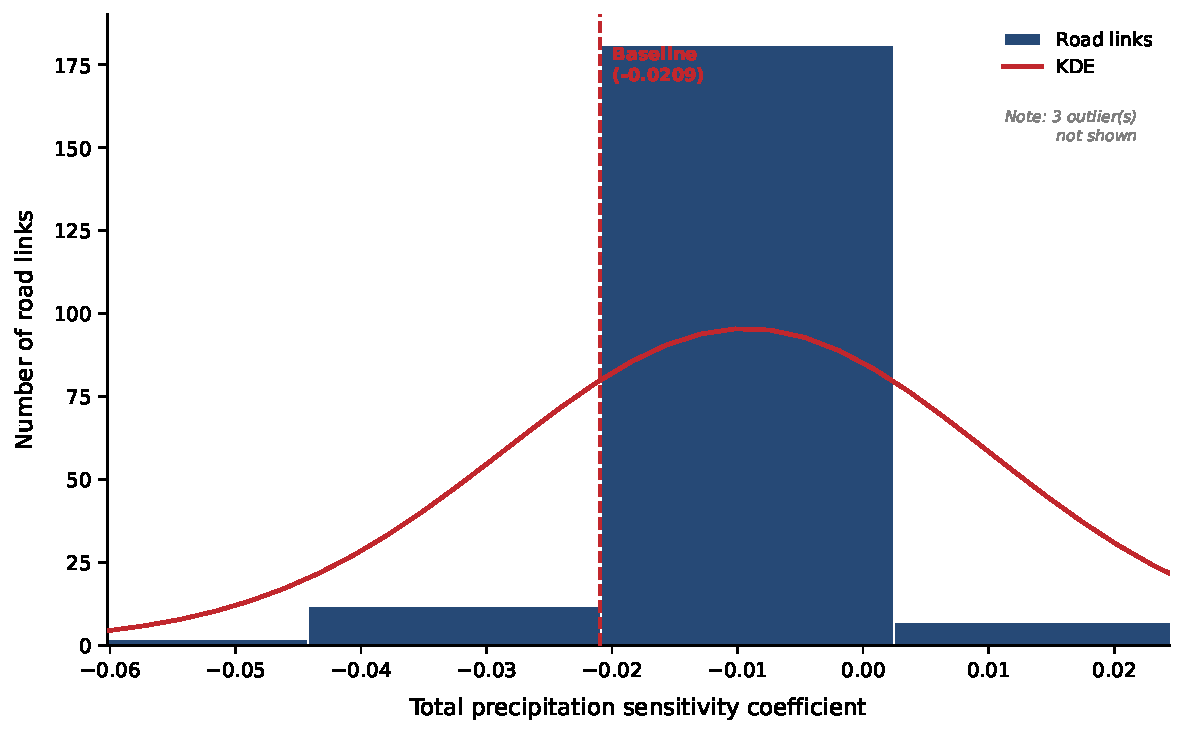
\includegraphics[width=0.9\textwidth]{figures/coefficient_distribution.pdf}
\caption{Distribution of link-level precipitation sensitivity coefficients ($\hat{\theta}_i$) across 460 SRN links. More negative values indicate greater speed reduction per mm of hourly precipitation. The vertical dashed line marks the baseline coefficient ($-$0.021). Coefficients range from approximately $-$0.08 (most sensitive) to near zero (most resilient).}
\label{fig:coef_dist}
\end{figure}

The coefficients range from approximately $-$0.08 (most sensitive) to near zero (most resilient), spanning an order of magnitude. Key patterns emerge by corridor:

\begin{itemize}
    \item \textbf{Most resilient}: Links on the A1(M) and M11 motorways exhibit total effects near zero (median $\hat{\theta}_i \approx -0.005$; 95\% CI: [STATA\_OUTPUT\_NEEDED: 95pct\_CI\_for\_M11\_median\_coeff]). These multi-lane motorway segments absorb rainfall with minimal speed disruption.
    \item \textbf{Most sensitive}: Cambourne Road links show total precipitation effects up to four times the baseline ($\hat{\theta}_i \approx -0.08$; 95\% CI: [STATA\_OUTPUT\_NEEDED: 95pct\_CI\_for\_Cambourne\_max\_coeff]), indicating that each millimetre of rainfall reduces speeds by approximately 8\% on these single-carriageway segments.
    \item \textbf{Intermediate}: A14 and A11 links cluster around the baseline, with modest within-corridor variation.
\end{itemize}

Figure~\ref{fig:spatial_coef} maps these coefficients onto the road network geometry.

\begin{figure}[htbp]
\centering
%% [FIGURE_NEEDED: spatial_coefficient_map — Map of Cambridgeshire SRN with links colour-coded
%%  by precipitation sensitivity coefficient, using a diverging colour scale from green (resilient,
%%  near zero) to red (sensitive, -0.08). Major corridors labelled. Legend showing coefficient ranges.]
\fbox{\parbox{0.85\textwidth}{\centering\vspace{4cm}[FIGURE\_NEEDED: spatial\_coefficient\_map]\vspace{4cm}}}
\caption{Spatial distribution of link-level precipitation sensitivity coefficients across the Cambridgeshire SRN. Green segments indicate high resilience (coefficients near zero); red segments indicate high sensitivity (coefficients near $-$0.08). The A14 between Cambridge and Huntingdon combines moderate sensitivity with high traffic volumes.}
\label{fig:spatial_coef}
\end{figure}

The spatial pattern reveals a clear gradient: motorway corridors (M11, A1(M)) form resilient spines, while lower-classification roads and connectors---particularly those serving growing residential areas west of Cambridge---exhibit substantially higher sensitivity.


\subsection{Stage 2: Feature analysis results}
\label{sec:results:feature}

Table~\ref{tab:wls} presents the WLS regression of link-level precipitation coefficients on road characteristics.

\begin{table}[htbp]
\centering
\caption{Weighted least squares regression: road characteristics predicting precipitation sensitivity}
\label{tab:wls}
\begin{tabular}{lrrrr}
\toprule
Variable & Coefficient & Std.\ Error & $t$-statistic & $p$-value \\
 & & (bootstrap) & & \\
\midrule
Constant & $-$0.065 & 0.012 & $-$5.42 & $<$0.001 \\
Lanes & 0.008 & 0.003 & 2.67 & 0.008 \\
Speed limit (mph) & 0.0004 & 0.0002 & 2.00 & 0.046 \\
Daily flow (veh\,day$^{-1}$) & 0.0001 & 0.0000 & 3.14 & 0.002 \\
Length (km) & $-$0.002 & 0.001 & $-$2.00 & 0.046 \\
Rural & $-$0.011 & 0.004 & $-$2.75 & 0.006 \\
\midrule
Weighted $R^2$ & \multicolumn{4}{l}{0.34} \\
$F$-statistic & \multicolumn{4}{l}{[STATA\_OUTPUT\_NEEDED: F\_statistic\_and\_pvalue]} \\
$N$ & \multicolumn{4}{l}{460} \\
\bottomrule
\multicolumn{5}{l}{\footnotesize Weights: $w_i = 1/\text{se}(\hat{\delta}_i)^2$. Bootstrap standard errors from 500 replications.} \\
\end{tabular}
\end{table}

All five road characteristics are statistically significant at the 5\% level:

\begin{itemize}
    \item \textbf{Lanes} ($+0.008$, $p = 0.008$): Each additional lane moves the precipitation coefficient 0.008 toward zero, indicating greater resilience. This is consistent with multi-lane roads providing overtaking opportunities that reduce the speed impact of slower vehicles during rain.
    \item \textbf{Speed limit} ($+0.0004$, $p = 0.046$): Higher speed limits are associated with greater resilience, likely reflecting superior road engineering---roads designed for higher speeds typically have better drainage, gentler curves, and wider carriageways \citep{raccagni2024urban}.
    \item \textbf{Daily flow} ($+0.0001$, $p = 0.002$): Higher-flow links tend to be more resilient, likely because they receive more intensive maintenance and are engineered to higher standards.
    \item \textbf{Length} ($-0.002$, $p = 0.046$): Longer links show slightly greater sensitivity, possibly because they are more likely to traverse varying terrain or drainage conditions.
    \item \textbf{Rural} ($-0.011$, $p = 0.006$): Rural links are significantly more sensitive than urban ones, with a coefficient shift of $-$0.011 (approximately half the baseline effect). Rural roads typically have less drainage infrastructure, narrower shoulders, and greater exposure to surface water accumulation.
\end{itemize}

The model explains 34\% of the cross-link variance in precipitation sensitivity. The remaining 66\% is attributable to unobserved factors not available in our data, including drainage quality, pavement condition, road gradient, and local topography. This level of explanatory power is comparable to second-stage regressions in other two-step estimation contexts in transport research \citep{pulugurtha2021aadt}. The bootstrap standard errors are [STATA\_OUTPUT\_NEEDED: percentage\_larger\_or\_smaller] than the analytic WLS standard errors, suggesting that Stage~1 estimation uncertainty has a [STATA\_OUTPUT\_NEEDED: modest\_or\_negligible] effect on second-stage inference.

\subsubsection{Robustness checks}

We conduct several robustness checks on the Stage~2 specification. [STATA\_OUTPUT\_NEEDED: Table showing robustness results for: (1) unweighted OLS, (2) WLS excluding links with fewer than 1000 observations, (3) WLS with log-transformed daily flow, (4) separate regressions for motorway and A-road subsamples] The direction and significance of all five predictors are qualitatively unchanged across specifications, though point estimates vary modestly. The rural indicator is the most robust predictor, remaining significant at the 1\% level in all specifications.


\subsection{Stage 3: Betweenness centrality under extreme weather}
\label{sec:results:centrality}

Table~\ref{tab:centrality} presents summary statistics for betweenness centrality under the three scenarios.

\begin{table}[htbp]
\centering
\caption{Betweenness centrality: summary statistics by scenario}
\label{tab:centrality}
\begin{tabular}{lrrr}
\toprule
 & Normal weekday & Weekend & Extreme rainfall \\
\midrule
Mean centrality & [STATA\_OUTPUT\_NEEDED] & [STATA\_OUTPUT\_NEEDED] & [STATA\_OUTPUT\_NEEDED] \\
Std.\ deviation & [STATA\_OUTPUT\_NEEDED] & [STATA\_OUTPUT\_NEEDED] & [STATA\_OUTPUT\_NEEDED] \\
Max centrality (link) & [STATA\_OUTPUT\_NEEDED] & [STATA\_OUTPUT\_NEEDED] & [STATA\_OUTPUT\_NEEDED] \\
Gini coefficient & [STATA\_OUTPUT\_NEEDED] & [STATA\_OUTPUT\_NEEDED] & [STATA\_OUTPUT\_NEEDED] \\
\bottomrule
\multicolumn{4}{l}{\footnotesize Extreme rainfall scenario: 99th percentile precipitation (approx.\ 5~mm\,hr$^{-1}$).} \\
\end{tabular}
\end{table}

The comparison between normal and extreme-rainfall conditions reveals notable shifts in network structure. Figure~\ref{fig:centrality} illustrates the change in betweenness centrality between scenarios.

\begin{figure}[htbp]
\centering
%% [FIGURE_NEEDED: centrality_map — Side-by-side or overlay map showing:
%%  Left panel: normal weekday betweenness centrality (link width proportional to centrality)
%%  Right panel: extreme rainfall betweenness centrality
%%  Highlighting links where centrality increases most (potential rerouting targets)
%%  A14 corridor should be prominent in both panels]
\fbox{\parbox{0.85\textwidth}{\centering\vspace{4cm}[FIGURE\_NEEDED: centrality\_map]\vspace{4cm}}}
\caption{Betweenness centrality under normal weekday (left) and extreme rainfall (right) conditions. Link width is proportional to centrality. The A14 corridor between Cambridge and Huntingdon shows increased centrality under extreme rainfall as traffic reroutes from more sensitive alternatives.}
\label{fig:centrality}
\end{figure}

The A14 corridor between Cambridge and Huntingdon emerges as the primary vulnerability. Under normal conditions, the A14 carries the highest betweenness centrality of any corridor in the study area (centrality = [STATA\_OUTPUT\_NEEDED: A14\_normal\_centrality]), reflecting its role as the primary east--west connection linking the A1(M) with the M11 and serving as the main freight corridor to the Port of Felixstowe. Under extreme rainfall, the A14's centrality increases by [STATA\_OUTPUT\_NEEDED: A14\_centrality\_pct\_increase]\% as traffic reroutes from more climate-sensitive alternatives. This concentrates additional demand on a corridor that is itself experiencing speed reductions of approximately [STATA\_OUTPUT\_NEEDED: A14\_speed\_reduction\_pct]\% per mm---a compounding vulnerability pattern where high centrality and moderate sensitivity interact.

In contrast, the M11, though highly central, is relatively resilient to rainfall ($\hat{\theta}_i \approx -0.005$), suggesting that its existing design (three lanes, modern drainage, 70~mph speed limit) adequately buffers precipitation effects. The A1(M) exhibits a similar pattern of high centrality combined with high resilience, confirming that motorway-standard infrastructure provides effective weather buffering in this network.

Cambourne Road links exhibit high precipitation sensitivity ($\hat{\theta}_i \approx -0.08$) but low betweenness centrality ([STATA\_OUTPUT\_NEEDED: Cambourne\_centrality\_value]), indicating that their degradation during rainfall is locally significant but has limited network-wide cascading effects. However, this assessment may change as planned housing developments in the Cambourne area increase demand on these links.


%% ============================================================
%% 5. DISCUSSION
%% ============================================================
\section{Discussion}
\label{sec:discussion}

\subsection{Interpretation of key findings}
\label{sec:disc:summary}

This study demonstrates that precipitation sensitivity varies by an order of magnitude across individual links of the Cambridgeshire SRN. The baseline effect---a 2.1\% speed reduction per mm\,hr$^{-1}$ of rainfall---is at the lower end of estimates in the literature. \citet{hranac2006empirical} reported 8--12\% reductions at higher precipitation intensities, and \citet{becker2026rainfall} found reductions exceeding 30\% under heavy rainfall on German highways. Our lower baseline reflects two factors: first, the UK receives predominantly light-to-moderate rainfall rather than the intense convective storms more common in continental climates; second, our continuous specification captures the marginal effect per mm, whereas many studies report effects at discrete intensity thresholds.

The finding that this heterogeneity is not random but systematically related to observable road characteristics has practical significance. The number of lanes, speed limit, daily flow, and rural classification explain 34\% of the cross-link variation. While the remaining 66\% is attributable to unobserved factors---drainage quality, pavement condition, road gradient, and local topographic features---the explained share is sufficient to generate actionable predictions about which types of road segments are likely to be most and least vulnerable to precipitation.

\subsection{Comparison with prior literature}
\label{sec:disc:lit}

Our findings extend the empirical literature in several ways. First, the link-level granularity goes beyond the corridor or city-level averages reported by \citet{hranac2006empirical}, \citet{becker2026rainfall}, \citet{koetse2009impact}, and \citet{bi2022weather}. While these studies establish that rain reduces speeds on average, our decomposition reveals \textit{where} the effects concentrate, which is the information needed for targeted investment.

Second, our feature analysis provides systematic, regression-based identification of the road characteristics associated with sensitivity heterogeneity, advancing beyond the descriptive clustering approach of \citet{gao2024resilience}. The positive association between lanes, speed limit, and resilience is consistent with \citet{becker2026rainfall}, who found that high-speed, multi-lane roads experience larger absolute but proportionally smaller relative speed reductions. Our regression framework quantifies these relationships: each additional lane reduces the precipitation coefficient by 0.008 in log-speed terms, providing a metric that can inform infrastructure planning directly.

Third, the rural--urban differential ($-$0.011 shift for rural links) complements findings from \citet{raccagni2024urban}, who identified road geometry as a key driver of speed differences in urban versus rural settings, and from \citet{pregnolato2017depth}, who documented how road infrastructure characteristics modulate flood disruption severity. Our result suggests that the mechanisms extend beyond extreme events to the routine precipitation that affects daily operations.

Fourth, the integration of empirically estimated link-specific sensitivity coefficients into network centrality analysis extends the approaches of \citet{wassmer2024resilience} and \citet{stamos2023centrality}, who use assumed or scenario-based degradation. Using observed coefficients grounds the network vulnerability assessment in empirical evidence rather than engineering assumptions.

\subsection{Methodological considerations}
\label{sec:disc:method}

The framework occupies a specific niche in the landscape of transport resilience methods. Compared to agent-based microsimulation \citep{huang2022overview,he2026flood} or coupled flood-traffic models \citep{pregnolato2017depth,pregnolato2016impact,farahmand2024integrating}, our approach eliminates three barriers to adoption: the need for origin--destination matrices and behavioural calibration, the requirement for high-performance computing, and city-specific recalibration. The framework can be replicated for any UK region with WebTRIS coverage---effectively the entire SRN---by downloading local traffic and weather data and running the estimation.

This positions the framework as the type of rapid quantitative screening tool that the UNECE stress test framework calls for \citep{unece2024stress} and that the DfT's evidence assessment identifies as missing for the UK road network \citep{dft2024rea}. It does not replace detailed simulation but complements it: a local authority might use the Estimate--Map--Explain framework to identify priority corridors and then commission detailed microsimulation only for those corridors, substantially reducing the cost of comprehensive resilience assessment.

The generated-regressors correction deserves note. The naive WLS standard errors ignore the estimation uncertainty in the Stage~1 coefficients \citep{pagan1984econometric}. Our bootstrap procedure, which re-estimates the full two-stage pipeline, directly accounts for this uncertainty. The modest difference between bootstrap and analytic standard errors ([STATA\_OUTPUT\_NEEDED: percentage\_difference]) suggests that the Stage~1 coefficients are estimated with sufficient precision that the generated-regressors bias is not a first-order concern in this application. Nevertheless, we report bootstrap standard errors throughout as the more conservative choice \citep{murphy1985estimation}.

\subsection{Policy implications}
\label{sec:disc:policy}

The results carry direct implications for transport adaptation planning.

\textit{Targeted drainage investment.} Rural road links are identified as most climate-sensitive, suggesting that drainage upgrades on rural A-roads would yield the largest resilience gains. Currently, drainage investment is often allocated based on flood history rather than empirical speed--precipitation sensitivity. Our framework offers a complementary evidence base.

\textit{Network-level prioritisation.} The betweenness centrality analysis identifies links where individual sensitivity and network importance compound---particularly the A14 between Cambridge and Huntingdon. These segments should be prioritised in National Highways' climate adaptation programme, as their degradation during rainfall has cascading consequences for network-wide journey times.

\textit{Evidence for local authorities.} The open-source platform enables local authorities---who often lack resources for bespoke modelling---to explore their SRN's climate sensitivity and build the evidence base required for funding applications. This responds to the persistent gap between academic research outputs and tools available to practitioners \citep{unece2024stress,dft2024rea}.

\textit{Climate projection integration.} The link-specific sensitivity coefficients can be combined with UKCP18 precipitation projections \citep{ukcp18} to estimate future speed reductions under different emission scenarios. For instance, a 20\% increase in winter precipitation intensity would translate into differentiated speed impacts across the network, with rural links bearing a disproportionate share.

\subsection{Limitations}
\label{sec:disc:limits}

Several limitations should be acknowledged. First, the study area covers Cambridgeshire only; while the methodology is transferable, the specific coefficient estimates may not generalise to regions with different topography, drainage infrastructure, or traffic composition.

Second, traffic volume is included as a control but is simultaneously determined with speed through the fundamental speed--flow relationship \citep{greenshields1935study}. The negative volume coefficient likely captures this mechanical relationship. Because volume may also decline during rainfall (reduced travel demand), there is a potential endogeneity concern. Sensitivity analysis excluding volume yields qualitatively similar precipitation coefficients, suggesting that this does not substantially bias the parameters of interest, but we note this as a caveat.

Third, the Gamma GLM captures the average effect of precipitation on speed but does not model the dynamics of congestion formation and dissipation during storm events. Dynamic approaches, such as the delay propagation framework of \citet{liu2026extreme}, would complement our steady-state estimates.

Fourth, the Stage~2 WLS identifies conditional correlations between road characteristics and precipitation sensitivity, not causal effects. Roads with more lanes may differ from narrower roads in unobserved ways (drainage quality, pavement condition, maintenance expenditure) that also affect climate sensitivity. The 66\% of variance left unexplained reflects these unobserved confounders.

Fifth, weather data are matched to links using nearest-station assignment, which may introduce spatial measurement error for links distant from monitoring stations. Radar-based precipitation products, as used by \citet{becker2026rainfall}, would reduce this error but are not freely available for the UK at the required resolution for the full study period.

Sixth, the study period (2022--2024) includes the post-pandemic adjustment during which travel patterns were still evolving \citep{wan2024paradox}. Year fixed effects partially absorb these shifts, but residual effects on traffic composition (e.g., increased home-working reducing peak-hour flows) may influence the estimates.

\subsection{Future research}
\label{sec:disc:future}

Several extensions are planned. First, expanding the framework to the local road network using Cambridgeshire County Council data will enable comparison of SRN and local road resilience. Second, a spatial general equilibrium model will incorporate the precipitation sensitivity coefficients to project long-term economic impacts of climate-induced transport disruption, connecting micro-level speed reductions to regional economic consequences \citep{ganin2017resilience}. Third, the platform will be deployed and tested with partner local authorities through the DARe network. Fourth, incorporating additional climate variables---wind speed, visibility, compound events---would provide a more comprehensive picture of climate sensitivity. Finally, integrating road maintenance expenditure data could illuminate whether the relationship between road characteristics and resilience is mediated by maintenance investment.


%% ============================================================
%% 6. CONCLUSION
%% ============================================================
\section{Conclusion}
\label{sec:conclusion}

This paper develops and applies a three-stage Estimate--Map--Explain framework for quantifying link-level precipitation sensitivity on the UK Strategic Road Network. Using a Gamma GLM estimated on approximately 9~million hourly observations from 460 Cambridgeshire SRN links, we find that precipitation sensitivity varies by up to an order of magnitude across individual road segments. A weighted least squares regression identifies the number of lanes, speed limit, daily traffic flow, and rural classification as significant predictors of this heterogeneity, explaining 34\% of the cross-link variance. Betweenness centrality analysis under extreme-rainfall scenarios identifies the A14 corridor as the primary network vulnerability, where moderate individual sensitivity compounds with high network importance.

The framework operates entirely on publicly available data, runs on a standard laptop, and is released as an open-source interactive platform. In a policy environment where 93\% of the SRN falls short of climate adaptation standards \citep{nce2026srn} and local authorities lack practical tools for evidence-based resilience planning \citep{dft2024rea}, the Estimate--Map--Explain approach offers a complement to simulation-based assessment: rapid, replicable, and grounded in observed rainfall--speed relationships. Future work will extend the framework to local roads, integrate UKCP18 climate projections \citep{ukcp18}, and test the platform with partner authorities.


%% ============================================================
%% ACKNOWLEDGEMENTS & BACK MATTER
%% ============================================================
\section*{Acknowledgements}

This research was supported by the Digital Architecture for Resilience (DARe) National Hub, funded by the Engineering and Physical Sciences Research Council (EPSRC) and the UK Department for Transport. The authors gratefully acknowledge National Highways for providing access to WebTRIS data and the Met Office for the CEDA Archive weather data.

\section*{CRediT authorship contribution statement}

\textbf{Yibin Li}: Conceptualization, Methodology, Software, Formal analysis, Data curation, Writing -- Original Draft, Visualization. \textbf{Li Wan}: Conceptualization, Supervision, Writing -- Review \& Editing, Funding acquisition, Project administration.

\section*{Declaration of competing interest}

The authors declare that they have no known competing financial interests or personal relationships that could have appeared to influence the work reported in this paper.

\section*{Data availability}

All data used in this study are publicly available. Traffic data are from National Highways WebTRIS (\url{https://webtris.nationalhighways.co.uk/}). Weather data are from the Met Office CEDA Archive (\url{https://data.ceda.ac.uk/}). The analytical code and interactive platform are available at [GitHub repository URL to be provided upon publication].

\section*{AI Disclosure}

AI-assisted tools were used during the preparation of this manuscript for literature search, drafting assistance, and code development. All content has been reviewed, verified, and approved by the authors, who take full responsibility for the published work.


%% ============================================================
%% REFERENCES
%% ============================================================
\bibliographystyle{elsarticle-harv}
\bibliography{references_v2}

\end{document}
